\chapter{System Implementation} \label{chap:Implementation}
This chapter is dedicated to the implementation details of the debugger. The first section describes the implementation method used in our chrome extension. In next section, we explain the data structures that capture all the data. In the third section, we explain how communication happens between different components of the extension. Finally, we discuss different components of the extension with the help of graphical user interface.

\section{Implementation method}
This section provides in-depth knowledge of how the chrome reactive inspector(CRI) is implemented.

 
\begin{figure}[!h]
	\centering
	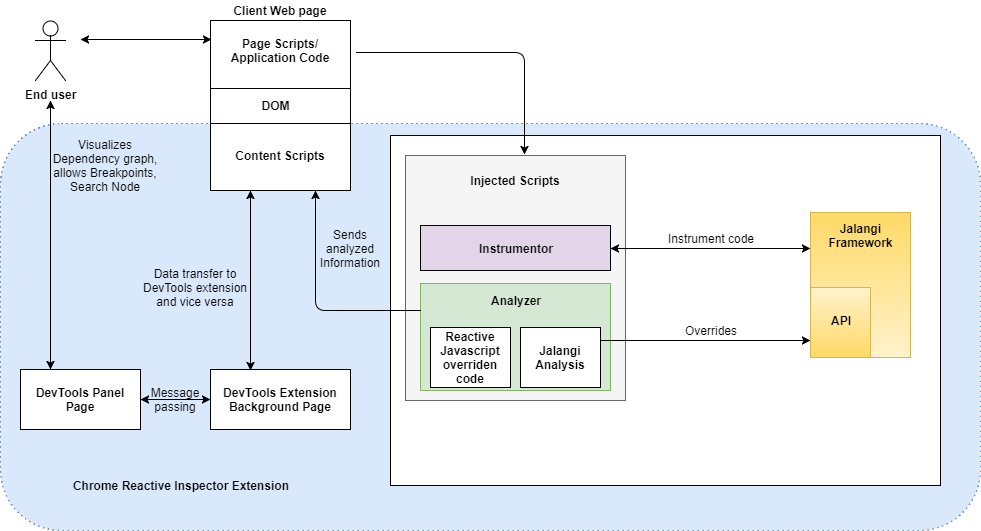
\includegraphics[width=\textwidth,height=\textheight,keepaspectratio]{images/detailed-system-implementation.png}
	\caption{Detailed System Components}
	\label{fig:detailed-system-implementation}
\end{figure}
As we explained earlier in the section \ref{section:extending_devtools}, current web page script and content script from extension have access to DOM. Figure~\ref{fig:detailed-system-implementation} depicts detailed system design. First, the user has to load a web page which contains reactive javascript code. Then open DevTools and select a panel \textit{Reactive Inspector}. The moment user selects the panel, we are then injecting two javascript files on-the-fly to our extension as shown in below code.


\begin{lstlisting}[language=JavaScript, caption=Injecting Javascript Files, label={lst:inject-javascript-files}]
chrome.tabs.executeScript(tabId, {file: "analyzer.js"}, function(){
	chrome.tabs.executeScript(tabId, {file: "instrumentor.js"}, function(){
		//all injected
	});
});
\end{lstlisting}

In the above code, file ``instrumentor.js'' works as a \textit{Interceptor}. Interceptor is responsible for loading all the client side javascript files sequentially and instrument them if required. Jalangi framework will help instrument all the javascript code. Then we evaluate instrumented code using \textit{eval()} function. The instrumented code invokes Jalangi API functions when it encounters operations such as reading a variable, reading a function etc. 

We override Jalangi API to catch all the operations performed by Jalangi framework. Analyzer component is responsible for further actions. It comprises of both overridden Jalangi API methods and catching all the events emitted by reactive libraries. Analyzer, with the help of Jalangi API, maps the reactive data streams to the respective variable names mentioned in the client code. Analyzer helps to catch the reactive library specific events such as creating an observable, subscriber subscribing to an observable, application of operators on observable, values emitted by observables etc. After catching the events, it analyzes them and then forwards the processed data to content-script. Content script then forwards it to background page and then finally it is forwarded to a panel in which an end user can see the generated dependency graph. All communication between content scripts, background page and panel are done via Message passing. Messages received by panel can be of type \textit{saveNode}, \textit{saveEdge} or \textit{sendAllNodesAndEdges}. In \textit{saveNode} message, we pass the node details such as nodeId, value, sourceCodeLine etc. and in \textit{saveEdge}, we specify between which nodes there should be a directed graph drawn in the graph. For each message received by the panel, the current state of the graph is saved for further computations such as traveling back and forth in history graph, history queries etc. Finally, a user can see the generated dependency graph, options to search nodes, find dependencies and add breakpoints. 

\section{Significant Data Structures for the Communication}
The three important data structures commonly used by the CRI are listed below:
\\
\textbf{Information about Reactive variables }
\\
Each node in the dependency graph contains following information.
\begin{itemize}
	\item nodeId: Each node in the graph is identified by unique Id
	\item nodeType: Every node in the graph are of type, which can be different kind of observables or subscribers in RxJS and eventStream or property in BaconJS.
	\item nodeRef: It contains variable name provided by user and identified by Jalangi. This can be empty in case of intermediate streams.
	\item nodeValue: It holds current values of respective variable.
	\item sourceCodeLine: It holds the line number of a variable which is defined in the client code and is identified by Jalangi.
\end{itemize}
\leavevmode
\\
\textbf{Data structure used in communication}
\\
Content script sends messages to panel vie background page to save node details and the edge details. To communicate, content script uses data structure defined in~\ref{lst:data-structure-1}. The \textit{action} attribute differentiates type of message, whether it is to save node details or save edge details. And \textit{destination} attribute is always set to \textit{panel} in our case.

\begin{lstlisting}[language=JavaScript, caption=Data structure for communication, label={lst:data-structure-1}]
// This data structure used in case of defining new reactive stream or updating the existing ones with new nodeValue
content: {
	'nodeId': '',
	'nodeType': '',
	'nodeRef': '',
	'nodeValue': '',
	'sourceCodeLine': ''
}, action: "saveNode", destination: "panel"

// This data structure used in case of defining a new dependency between two reactive streams
content: {
	"edgeStart": '',
	"edgeStartName": '',
	"edgeEnd": '',
	"edgeEndName": '',
	"edgeLabel": ''
},
action: "saveEdge",
destination: "panel"

\end{lstlisting}

To send edge details, we define another data structure as presented in the listing ~\ref{lst:data-structure-1}. Each attribute are defined as follows:
\begin{itemize}
	\item edgeStart: It denotes the parent node on which another node depends on. 
	\item edgeStartName: It holds name of parent node. 
	\item edgeEnd: It  denotes the child node which is subscribed to parent node.
	\item edgeEndName: It holds name of child node.
	\item edgeLabel: It denotes how parent and child node are related. 
\end{itemize}
\leavevmode
\\
\textbf{History entry}
\\
For history queries feature, we need to save all the events happening in CRI. The data structure used for this purpose is defined in listing~\ref{lst:data-structure-2}.

\begin{itemize}
	\item stageId: It holds value which defines current stage number.
	\item type: It holds type of history entry such as \textit{dependencyCreated} etc.
	\item nodeName: holds node name in string form.
	\item nodeId: It holds id of the node.
	\item nodeValue: It holds value of node at that point of time.
\end{itemize}

\begin{lstlisting}[language=JavaScript, caption=History entry Data structure, label={lst:data-structure-2}]
historyEntry = {
	'stageId': '',
	'type': '',
	'nodeName': '',
	'nodeId':'',
	'nodeValue': ''
}

\end{lstlisting}
\leavevmode
\section{Communication between components}
The building block of components working together is communication. We know that content scripts and other scripts of an extension run in the different context of the plugin. In CRI, content scripts include interceptor and analyzer. These need a way to communicate with the panel where dependency graph is displayed and a user can interact with it. Also for every new message, dependency graph should be updated. Chrome provides two ways of communication APIs.  One way is using simple API for one-time requests\footnote{\url{https://developer.chrome.com/apps/messaging\#simple} , last accessed 13-09-2017} and another is using complex API that allows long-lived connections\footnote{\url{https://developer.chrome.com/apps/messaging\#connect} , last accessed 13-09-2017}. Since content scripts and background page needs to communicate continuously, we use long-lived connections. When a user opens DevTools, background script opens up a unique port for the panel named \textit{Reactive-Inspector} and adds message listeners to receive messages from background script. The code mentioned in listing \ref{lst:panel-background} is executed when an user opens DevTools. Here, it is creating a panel and creating a channel to post a message to the background page.

\begin{lstlisting}[language=JavaScript, caption=Creating a channel for communication between Panel and Background pages, label={lst:panel-background}]
//Creates a panel with name "Reactive-Inspector" in DevTools
chrome.devtools.panels.create("Reactive-Inspector", "reactive-debugger.png", "panel.html", function (extensionPanel) {
	// Opens a port with unique port number for the created panel
	var port = chrome.runtime.connect({name: 'Reactive-Inspector'});
	// this listens to any messages sent by background page
	port.onMessage.addListener(function(msg) {
	// Perform the actions on received messages such as
	// creating new or updating existing variable, dependency created etc.
	});
});

\end{lstlisting}

Similarly, there should be another channel for background script to communicate with panel script. Listing \ref{lst:background-panel} contains the relevant code snippet. Here, we set up a channel to receive messages sent to background script as shown in line 46. When DevTools with CRI is opened in two different browser tabs, it is hard to differentiate panels by panel name because both panels have the same name. Hence to differentiate between panels of different tabs, we need to store port numbers of both panels to avoid cross panel communication. 
\begin{lstlisting}[language=JavaScript, caption=Channel for background script to communicate with Panel script, label={lst:background-panel}]
// holds objects of key-value pairs of tabid and port number
var tabPorts = {};

// creates a listener to listen to messages sent by Panel script
chrome.runtime.onConnect.addListener(function (port) {
	
	var tabId;
	port.onMessage.addListener(function(message){
		if (!tabId) {
			// add tabId to each message
			tabId = message.tabId;
			// maps port number to tabId
			tabPorts[tabId] = port;
		}
		// explained in section 4.1
		chrome.tabs.executeScript(tabId, {file: "analyzer.js"}, function(){
			chrome.tabs.executeScript(tabId, {file: "instrumentor.js"}, function(){
				//all injected
			});
		});
	});
	
	// function called for every message received by background page
	var extensionListener = function (message, sender, sendResponse) {
		// holds current port number		
		const port = sender.tab && tabPorts[sender.tab.id];
		// if port is open and message destination is 'panel', forward message to Panel
		if (port && message.destination === "panel") {
			port.postMessage(message);
		} else {
			// if no destination provided, forward message to content script
			if (message.tabId && message.content) {
				chrome.tabs.sendMessage(message.tabId, message, sendResponse);
			} else {
			if(port)
				// if no tabId, then forward message to panel from content script
				port.postMessage(message);
				else
				return false;
			}	
		}
		sendResponse(message);
	};
	
	// Listens to messages sent from the panel
	chrome.runtime.onMessage.addListener(extensionListener);
	
	// listener to DevTools disconnection
	port.onDisconnect.addListener(function (port) {
		// remove port number when DevTools is disonnected and remove listener for message receivers
		delete tabPorts[tabId];
		chrome.extension.onMessage.removeListener(extensionListener);
	});
});

// Deletes current port when current browser tab is closed
chrome.tabs.onRemoved.addListener(function (tabId) {
	delete tabPorts[tabId];
});

\end{lstlisting}

\section{CRI User Interface} \label{section:cri-ui}
The user interface(UI) of the CRI is a panel which can be seen when user opens chrome DevTools. After opening DevTools, CRI can be activated by clicking on ``Reactive-Inspector'' panel. The UI can be divided into 6 main parts as shown in Figure~\ref{fig:cri}. 

\begin{figure}[!h]
	\centering
	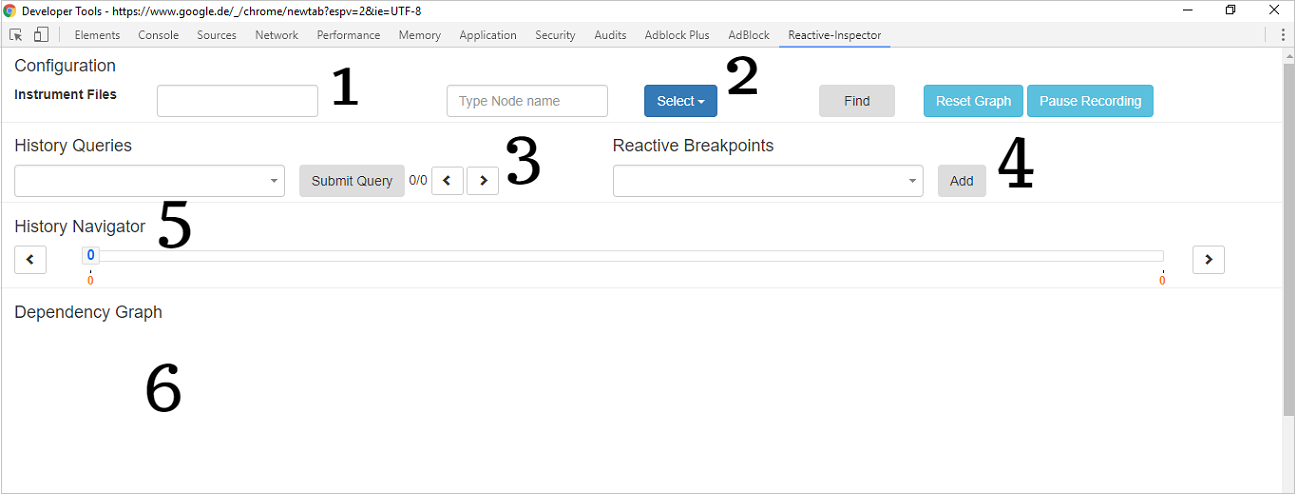
\includegraphics[scale=0.5,trim=0 0 0 0]{images/cri.png}
	\caption{Chrome Reactive Inspector}
	\label{fig:cri}
\end{figure}

\leavevmode
\\
\textbf{Part 1 - Scoping Feature}
\\
This view is responsible for \textit{Scoping} feature. The user can mention which files to be included for instrumenting by Jalangi framework. For example, if a user enters file named 'index.js', only this file will be instrumented and other files are excluded. It is an optional feature. If the field is empty, then Jalangi instruments all the client-side javascript files. 

\leavevmode
\\
\textbf{Part 2 - Node details}
\\
This view is responsible for 3 features: search node by name, find dependents of the given node and find dependencies of a node. The user can select which feature he/she wants to use and click on Find button. 
The results will be shown in the dependency graph. 

\leavevmode
\\
\textbf{Part 3 - History Queries}
\\
The user can use this part to query all the history entries. We use query language for querying the history. When expanded, the views looks as shown in the Figure \ref{fig:language-query}. The user can select any one of the options and edit it as per the requirement. For instance, to query creation of node named 'x', user selects an option \textit{NodeCreated} and edit it to \textit{NodeCreated[x]}.
\begin{figure}[!h]
	\centering
	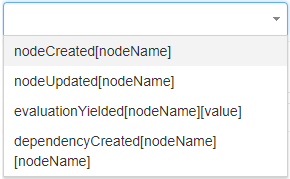
\includegraphics[scale=1,trim=0 0 0 0]{images/language-query.png}
	\caption{History Query}
	\label{fig:language-query}
\end{figure}

\leavevmode
\\
\textbf{Part 4 - Reactive Breakpoints}
\\
This feature is responsible for adding or removing reactive breakpoints. This looks similar to figure \ref{fig:language-query} but we use nodeId instead of nodeName for queries. The user selects an option and clicks on Add button to add a new breakpoint. List of all the current breakpoints is displayed right side of the button. The user can remove breakpoints if they are not required anymore.

\leavevmode
\\
\textbf{Part 5 - History Navigator}
\\
To navigate to and forth between the history of the dependency graph evolution, we have provided a slider. A user can either slide the slider or use the buttons < or > to navigate. 

\leavevmode
\\
\textbf{Part 6 - Dependency Graph}
\\
This view is responsible to display the current state of a dependency graph. Dependency graph updates as soon as there is a new event. Each node in the graph provides node details such as nodeId, name, current value and source code line number. Additionally, a user can mouse hover on each node for more details on a particular node. The dependency graph is visualized with the help of open source javascript library called dagre-d3\cite{dagred3}. By default, the library provides zoom in and zoom out functionality for the graph. We have also added a new feature to print node details to console when a user clicks a node. 